% Options for packages loaded elsewhere
\PassOptionsToPackage{unicode}{hyperref}
\PassOptionsToPackage{hyphens}{url}
\documentclass[
  10pt,
  twocolumn]{article}
\usepackage{xcolor}
\usepackage[margin=1.6cm]{geometry}
\usepackage{amsmath,amssymb}
\setcounter{secnumdepth}{-\maxdimen} % remove section numbering
\usepackage{iftex}
\ifPDFTeX
  \usepackage[T1]{fontenc}
  \usepackage[utf8]{inputenc}
  \usepackage{textcomp} % provide euro and other symbols
\else % if luatex or xetex
  \usepackage{unicode-math} % this also loads fontspec
  \defaultfontfeatures{Scale=MatchLowercase}
  \defaultfontfeatures[\rmfamily]{Ligatures=TeX,Scale=1}
\fi
\usepackage{lmodern}
\ifPDFTeX\else
  % xetex/luatex font selection
  \setmainfont[]{Times New Roman}
\fi
% Use upquote if available, for straight quotes in verbatim environments
\IfFileExists{upquote.sty}{\usepackage{upquote}}{}
\IfFileExists{microtype.sty}{% use microtype if available
  \usepackage[]{microtype}
  \UseMicrotypeSet[protrusion]{basicmath} % disable protrusion for tt fonts
}{}
\makeatletter
\@ifundefined{KOMAClassName}{% if non-KOMA class
  \IfFileExists{parskip.sty}{%
    \usepackage{parskip}
  }{% else
    \setlength{\parindent}{0pt}
    \setlength{\parskip}{6pt plus 2pt minus 1pt}}
}{% if KOMA class
  \KOMAoptions{parskip=half}}
\makeatother
\usepackage{longtable,booktabs,array}
\newcounter{none} % for unnumbered tables
\usepackage{calc} % for calculating minipage widths
% Correct order of tables after \paragraph or \subparagraph
\usepackage{etoolbox}
\makeatletter
\patchcmd\longtable{\par}{\if@noskipsec\mbox{}\fi\par}{}{}
\makeatother
% Allow footnotes in longtable head/foot
\IfFileExists{footnotehyper.sty}{\usepackage{footnotehyper}}{\usepackage{footnote}}
\makesavenoteenv{longtable}
\usepackage{graphicx}
\makeatletter
\newsavebox\pandoc@box
\newcommand*\pandocbounded[1]{% scales image to fit in text height/width
  \sbox\pandoc@box{#1}%
  \Gscale@div\@tempa{\textheight}{\dimexpr\ht\pandoc@box+\dp\pandoc@box\relax}%
  \Gscale@div\@tempb{\linewidth}{\wd\pandoc@box}%
  \ifdim\@tempb\p@<\@tempa\p@\let\@tempa\@tempb\fi% select the smaller of both
  \ifdim\@tempa\p@<\p@\scalebox{\@tempa}{\usebox\pandoc@box}%
  \else\usebox{\pandoc@box}%
  \fi%
}
% Set default figure placement to htbp
\def\fps@figure{htbp}
\makeatother
\setlength{\emergencystretch}{3em} % prevent overfull lines
\providecommand{\tightlist}{%
  \setlength{\itemsep}{0pt}\setlength{\parskip}{0pt}}
\usepackage{bookmark}
\IfFileExists{xurl.sty}{\usepackage{xurl}}{} % add URL line breaks if available
\urlstyle{same}
\hypersetup{
  pdftitle={Structural Determinants Without Short-Term Predictability: A Leakage-Controlled Benchmark of State-Level Dengue Burden in India{,} 2015--2024},
  pdfauthor={Siddalingaiah H S\^{}\{1,*\}; Sowjanya D\^{}\{1\}; Rangaswamy H V\^{}\{1\}},
  hidelinks,
  pdfcreator={LaTeX via pandoc}}

\title{Structural Determinants Without Short-Term Predictability: A
Leakage-Controlled Benchmark of State-Level Dengue Burden in India,
2015--2024}
\author{Siddalingaiah H S\(^{1,*}\) \and Sowjanya
D\(^{1}\) \and Rangaswamy H V\(^{1}\)}
\date{}

\begin{document}
\maketitle
\begin{abstract}
\textbf{Background:} Machine-learning early-warning systems for dengue
are proliferating, and many report high predictive accuracy. Such claims
are fragile: they depend entirely on the provenance of the underlying
surveillance data and on whether the evaluation design excludes
information that would not be available at the moment a forecast is
issued. India, which carries a large share of the global dengue burden,
has been a frequent subject of these models, yet no continuous monthly
state-level case series is publicly available for the country.
\textbf{Objectives:} To (i) assemble and independently verify an
authentic state-level dengue panel for India; (ii) establish, under a
strictly leakage-free design, how much genuine one-year-ahead predictive
skill is attainable and whether machine learning improves on elementary
baselines; (iii) quantify how far two common design defects --- an
unshifted rolling target statistic and non-temporal validation ---
inflate apparent performance; and (iv) test whether structural
vulnerability indicators explain the between-state burden landscape.
\textbf{Methods:} We compiled every observed annual state-level dengue
total released by India's National Centre for Vector Borne Diseases
Control (NCVBDC) and archived by OpenDengue for 2015--2024. Only states
with an observed value in all ten years were retained; nothing was
interpolated, imputed or reconstructed from higher-level totals. The
resulting panel of \textbf{350 state-years across 35 states and union
territories} was cross-checked against the independent NCVBDC bulletin.
Structural covariates comprised the NITI Aayog Health Index (2019-20),
state GDP per capita, the State Energy \& Climate Index, Census 2011
urban share and population density. Forecasts of year \emph{t} used only
information observable to 31 December \emph{t}−1. Seven models ---
persistence, state climatology, a global annual mean, negative-binomial
GLMs and gradient-boosting ensembles --- were compared on identical
expanding-window splits (origins 2018--2024; 245 out-of-sample
forecasts). We report pooled and within-state (state-mean-removed) R²,
out-of-fold permutation importance, and, for outbreak-year
classification, AUC-ROC, precision--recall, Brier score and calibration
with thresholds derived inside each training window. \textbf{Results:}
All 124 overlapping state-years reconciled \textbf{exactly} with the
NCVBDC bulletin (100\% agreement). No machine-learning model
outperformed elementary baselines: state climatology achieved the
highest pooled R² (\textbf{0.637}), ahead of a negative-binomial GLM
(0.607), gradient boosting (0.551) and persistence (0.550). Critically,
\textbf{within-state R² was approximately zero or negative for every
model} (best −0.002; gradient boosting −0.239), showing that pooled
skill reflects only the recovery of stable between-state differences in
burden, not anticipation of temporal change. Outbreak-year
classification was uninformative (AUC 0.522; average precision 0.468
against a prevalence of 0.452; Brier 0.326, worse than the
non-informative baseline of 0.248). Reintroducing an unshifted
three-year rolling mean raised apparent R² from 0.551 to \textbf{0.759},
and non-temporal random-split validation raised it to 0.626. By
contrast, the between-state structural gradient was strong and robust:
mean annual incidence rose with urbanisation (Spearman ρ =
\textbf{0.635}, 95\% CI 0.33--0.82, p \textless{} 0.001) and GDP per
capita (ρ = \textbf{0.609}, 95\% CI 0.32--0.80, p \textless{} 0.001),
the latter persisting after adjustment for a surveillance-capacity proxy
(partial ρ = 0.663, p \textless{} 0.001). The NITI Health Index showed
no association (ρ = 0.159, p = 0.38). \textbf{Conclusions:} On
authenticated Indian surveillance data, state-level dengue burden one
year ahead is \textbf{not} predictable beyond a state's own historical
average, and outbreak-year classification performs at chance. Reported
accuracies substantially above this level should be treated as evidence
of design leakage rather than of epidemiological signal. Where dengue in
India \emph{is} systematically patterned is spatially: burden
concentrates in more urbanised and more economically developed states.
Surveillance investment and vector control should therefore be allocated
on structural and demographic grounds rather than on the promise of
short-horizon algorithmic forecasting at this spatial and temporal
resolution. \textbf{Keywords:} Dengue; India; Data leakage; Forecast
evaluation; Benchmarking; Negative results; Surveillance data
provenance; Public-health informatics
\end{abstract}

\subsection{1. Introduction}\label{introduction}

\subsubsection{1.1 The Global and National Burden of
Dengue}\label{the-global-and-national-burden-of-dengue}

Dengue, caused by four serotypes of the \emph{Flaviviridae} virus (DENV
1--4), is the most rapidly spreading mosquito-borne viral disease
globally; the World Health Organization estimates a 30-fold rise in
incidence over the past five decades, placing nearly half the world's
population at risk \textsuperscript{1}. India, with its tropical climate
and dense, rapidly urbanising population, bears a disproportionate share
--- an estimated one-third of the global burden, likely underestimated
by passive surveillance \textsuperscript{2}. Inter-epidemic intervals
have narrowed in recent years, while the economic cost runs into
billions of dollars annually \textsuperscript{3}.

\subsubsection{1.2 Prediction Claims and Their Dependence on
Design}\label{prediction-claims-and-their-dependence-on-design}

Control in India rests on the NCVBDC \textsuperscript{4} and the
Integrated Disease Surveillance Programme, systems designed for
retrospective case reporting rather than prediction. This gap has
motivated a large modelling literature, from climate-driven seasonal
forecasting services \textsuperscript{5} to machine-learning outbreak
classifiers, much of it reporting high accuracy --- coefficients of
determination above 0.85 and near-unity outbreak AUCs are common
\textsuperscript{6}.

Two considerations should temper the reading of such results. The first
is \textbf{provenance}. A predictive claim about India presupposes a
case series at the claimed spatial and temporal resolution. NCVBDC
publishes state-wise totals annually; OpenDengue, the principal open
archive of global dengue counts \textsuperscript{7}, contains for India
only annual admin-1 records together with a single year of national
monthly values. Where monthly state-level series appear in the
literature, they are frequently reconstructed by distributing annual
totals across months using an assumed seasonal profile. Any model
trained on such a series will recover that assumed profile, and the
resulting ``seasonality is the dominant driver'' finding is an artefact
of the reconstruction rather than a discovery about transmission.

The second is \textbf{temporal validity}. A forecast is only a forecast
if every predictor was observable before the target period began.
Rolling statistics computed without first lagging the outcome series
embed the target inside the predictor matrix; outbreak thresholds
estimated on the whole study period leak future information into the
definition of the label; and random-split cross-validation abolishes the
temporal ordering that makes the task difficult. Each defect inflates
apparent performance without improving prospective utility, and leakage
of exactly these kinds has been identified as a leading cause of
irreproducible findings across machine-learning-based science
\textsuperscript{8}.

\subsubsection{1.3 The Structural Vulnerability
Hypothesis}\label{the-structural-vulnerability-hypothesis}

Beyond climate and epidemic momentum, dengue is shaped by the human and
systemic environment: it is an urban disease, amplified by water-storage
practices and sanitation failures, and \emph{detected} burden is
filtered through the strength of each state's health system. We
therefore examine whether structural indicators --- the NITI Aayog
Health Index \textsuperscript{9}, GDP per capita, the State Energy \&
Climate Index, urbanisation and population density --- explain the
burden landscape. We stress at the outset that reported cases are not a
direct measure of health-system weakness: stronger systems may record
\emph{more} cases through better diagnosis and surveillance, while
weaker systems may under-report a greater true burden. This design can
identify predictive and between-state associations; it cannot establish
a causal vulnerability--exposure mechanism.

\subsubsection{1.4 Objectives}\label{objectives}

We set out to establish what an authenticated Indian dengue panel
actually supports. Our hypothesis --- that combining epidemiological
history with structural indicators would improve prediction --- is
stated here as the hypothesis the study tested. As Section 3 reports, it
was \textbf{not} supported, and we present that outcome rather than a
favourable reformulation of it. Alongside the negative forecasting
result we report a formal leakage experiment that quantifies how large
the corresponding optimistic bias would have been, and a between-state
analysis that locates where systematic structure in Indian dengue does
exist.

\begin{center}\rule{0.5\linewidth}{0.5pt}\end{center}

\subsection{2. Methods}\label{methods}

\subsubsection{2.1 Study Design and
Reporting}\label{study-design-and-reporting}

This is a retrospective, longitudinal ecological modelling study at the
state--year level; the analytical unit is the ``state-year.'' Reporting
follows TRIPOD+AI \textsuperscript{10}: we specify data sources and
their provenance, the full predictor set, model configuration, the
forecast origin, validation procedure, discrimination \emph{and}
calibration with uncertainty, and we release code and data (Section
2.9). Because all data are aggregate, anonymised and publicly available,
individual ethics approval was not required (Section 2.10).

\subsubsection{2.2 Data Provenance}\label{data-provenance}

Case data are the observed annual state-level dengue totals reported by
NCVBDC \textsuperscript{4} and archived in the OpenDengue Spatial
extract V1.3 \textsuperscript{7}. We retained records with
\texttt{adm\_0\_name\ =\ INDIA}, \texttt{S\_res\ =\ Admin1},
\texttt{T\_res\ =\ Year} and a \texttt{MOH-IND} source identifier,
giving 358 state-year records for 2015--2024 across 41 administrative
labels. State names were harmonised to a canonical list (for example
ORISSA → ODISHA, PONDICHERRY → PUDUCHERRY). Where a state-year appeared
under more than one ministry release, the revised return superseded the
provisional one; no duplicate was summed.

We deliberately did \textbf{not} attempt to construct a monthly series.
No continuous monthly admin-1 dengue series exists in the public domain
for India: OpenDengue holds only 12 monthly records for the country, all
national and all from 2024. Annual data are therefore the finest
resolution at which an authentic Indian state-level panel can be
assembled, and the study is specified at that resolution.

\subsubsection{2.3 Eligibility and
Exclusions}\label{eligibility-and-exclusions}

A state or union territory was eligible only if an observed NCVBDC total
was present for \textbf{every} one of the ten study years. No missing
year was imputed, interpolated or carried forward. Thirty-five of 36
candidate states and union territories met this criterion, yielding
\textbf{350 state-years}. One state, West Bengal, was excluded for two
missing years. Six state-years carry genuine zero counts; these are true
reported zeros in small union territories and were retained as observed.
Panel construction, the eligibility rule and the full exclusion record
are tabulated in \textbf{Supplementary Table S1}. Because eligibility is
defined solely by completeness of the annual return, the
surveillance-related selection pressure is far weaker than in designs
that require continuous monthly reporting, but it is not absent, and we
address it in Section 4.5.

\subsubsection{2.4 Independent
Reconciliation}\label{independent-reconciliation}

To verify that the panel reproduces the official record rather than a
derived approximation, we cross-checked it against the NCVBDC state-wise
annual bulletin, which overlaps the panel for 2021--2024. All
\textbf{124 of 124} overlapping state-years matched exactly (100\%;
median absolute difference 0.0\%). The full reconciliation table is
provided as \textbf{Supplementary Table S2} and plotted in
\textbf{Figure 1B}.

\subsubsection{2.5 Structural Covariates}\label{structural-covariates}

Five time-invariant state-level indicators were merged by harmonised
name: the NITI Aayog Health Index 2019-20, a composite 0--100 score of
health outcomes, governance and inputs \textsuperscript{9}; state GDP
per capita; the NITI State Energy \& Climate Index (round 1); the Census
2011 urban population share; and Census 2011 population density.
Population was additionally used as a log offset in count models.
Coverage gaps were confined to three small union territories (Daman \&
Diu, Dadra \& Nagar Haveli, Lakshadweep); these were median-imputed
\textbf{and flagged}, and every between-state association in Section 3.4
is computed on states with observed covariates only (n = 32). No climate
covariates were included: state-resolution meteorological fields
matching the full 2015--2024 window were not available to us at annual
resolution, and we prefer to omit a block outright rather than
reconstruct it. Annual aggregation would in any case obscure the
sub-seasonal temperature dependence through which climate acts on
transmission, the extrinsic incubation period shortening from roughly 12
days at 25 °C to 7 days at 30 °C \textsuperscript{11}. This is stated as
a limitation in Section 4.5.

\subsubsection{2.6 Forecast Origin and Feature
Construction}\label{forecast-origin-and-feature-construction}

The forecasting task is explicit: \textbf{using only information
observable up to 31 December of year \emph{t}−1, predict the reported
dengue case total of year \emph{t}}. Predictors comprise cases in years
\emph{t}−1 and \emph{t}−2 (log-transformed), the year-on-year log growth
rate between them, and the expanding mean and maximum of all prior years
--- each formed by lagging the outcome series \emph{before} any rolling
or expanding statistic is computed --- together with the five structural
covariates and log population. Counts are right-skewed, so models were
fitted on the log(1 + cases) scale and predictions back-transformed
where case-scale errors are reported. Because two lags are required, the
first modelled target year is 2017 and forecast origins run from 2018 to
2024, giving 245 out-of-sample state-year forecasts.

\subsubsection{2.7 Benchmarks, Validation and
Metrics}\label{benchmarks-validation-and-metrics}

All models were evaluated on \textbf{identical expanding-window splits}:
for each target year, training used every eligible state-year strictly
before it. We compared seven specifications:

\begin{enumerate}
\def\labelenumi{\arabic{enumi}.}
\tightlist
\item
  \textbf{Persistence} --- the previous year's count.
\item
  \textbf{State climatology} --- the state's mean count over the
  training window only.
\item
  \textbf{Global annual mean} --- a single national constant.
\item
  \textbf{Negative-binomial GLM (history)} --- log-lagged counts with a
  log-population offset.
\item
  \textbf{Negative-binomial GLM (full)} --- as above plus structural
  covariates.
\item
  \textbf{Gradient boosting (history only)} \textsuperscript{12} --- 300
  trees, depth 2, learning rate 0.05, subsample 0.9.
\item
  \textbf{Gradient boosting (multi-modal)} --- identical configuration
  on history plus structural covariates.
\end{enumerate}

Hyperparameters were fixed a priori rather than tuned against the
evaluation folds. We report pooled R² on the log scale, MAE and RMSE on
the case scale, and mean per-origin R².

Because pooling states with very different baseline burdens can inflate
R² through recovery of state means alone, we additionally report a
\textbf{within-state R²}, computed after subtracting each state's
training-window mean from both observed and predicted values. This
isolates the component of skill that concerns temporal change, and the
state climatology baseline provides the explicit ``state mean only''
comparator. Performance disaggregated by state is reported in
\textbf{Supplementary Table S3}, and the complete metric set for every
specification in \textbf{Supplementary Table S4}.

\subsubsection{2.8 Outbreak-Year
Classification}\label{outbreak-year-classification}

An ``outbreak year'' is a state-year exceeding that state's 75th
percentile of reported cases. Critically, this threshold was recomputed
\textbf{inside each training window} rather than over the full panel, so
the label definition never uses future data. The decision cut-off
applied to the test year was likewise chosen by maximising Youden's J on
the \emph{training} predictions only. We report AUC-ROC, average
precision against the observed prevalence, the Brier score against a
non-informative baseline, a quintile calibration curve, and sensitivity,
specificity and PPV at the training-derived cut-off. Reporting
discrimination alongside calibration and a prevalence-referenced
precision measure, rather than AUC-ROC alone, follows current guidance
on evaluation metrics for medical applications of artificial
intelligence \textsuperscript{13}.

\subsubsection{2.9 Interpretability}\label{interpretability}

Impurity-based (``Gini'') importance is biased when predictors are
correlated and does not indicate the direction of an effect. We
therefore report \textbf{out-of-fold permutation importance}: for each
forecast origin, each predictor in the held-out year is permuted 30
times and the resulting increase in out-of-sample MAE recorded. Values
are averaged across origins and aggregated into two blocks ---
epidemiological history and structural vulnerability. These are
predictive importances, not causal contributions.

\subsubsection{2.10 Between-State
Associations}\label{between-state-associations}

State-level associations were estimated by Spearman correlation between
each structural covariate and each of three outcomes --- mean annual
incidence per 100 000, mean annual cases and cumulative cases --- with
95\% confidence intervals from 4 000 bootstrap resamples. Incidence is
the primary outcome because raw counts largely track population size. To
address the concern that wealthier states may report more cases simply
because they detect more, we additionally computed the partial Spearman
correlation between GDP per capita and incidence adjusting for the NITI
Health Index as a proxy for detection and reporting capacity.

\subsubsection{2.11 Leakage Experiment}\label{leakage-experiment}

To quantify the optimistic bias produced by common design defects, we
re-ran the identical pipeline on the identical real data under three
additional specifications: (a) adding a three-year rolling mean computed
\textbf{without} lagging the outcome, so that it contains the target
year; (b) replacing temporal splits with five-fold random-split
cross-validation; and (c) defining outbreak thresholds on the full panel
rather than the expanding training window. Differences from the primary
specification measure the inflation attributable to each defect. The
specification of each variant is set out in \textbf{Supplementary Table
S5}.

\subsubsection{2.12 Software and
Reproducibility}\label{software-and-reproducibility}

Analyses used Python 3 with scikit-learn, pandas, NumPy, SciPy,
statsmodels, GeoPandas and Matplotlib. The analysis panel, the
reconciliation table and the complete modelling, validation and figure
code are openly available (see Availability of Data and Materials), and
regenerate every number and figure reported here in a single pass from
the archived public source files. Step-by-step reproduction
instructions, together with checksums for every input, are given in
\textbf{Supplementary Table S6}.

\subsubsection{2.13 Ethics}\label{ethics}

The study used only aggregated, anonymised, publicly available
state-level data and involved no individual participants; institutional
ethics approval and consent were not applicable.

\begin{center}\rule{0.5\linewidth}{0.5pt}\end{center}

\subsection{3. Results}\label{results}

\subsubsection{3.1 An Authenticated Panel}\label{an-authenticated-panel}

The analysis panel comprises \textbf{350 state-years across 35 states
and union territories, 2015--2024}. Reported national totals rise from
91 397 cases in 2015 to a peak of 258 552 in 2023, interrupted by a
pronounced fall to 39 419 in 2020 (\textbf{Figure 1A}) --- consistent
with the documented collapse in dengue case detection across the
South-East Asia region during the COVID-19 pandemic
\textsuperscript{14}, a disruption that any authentic Indian
surveillance series must display. All 124 state-years overlapping the
independent NCVBDC bulletin matched exactly (\textbf{Figure 1B}),
confirming that the panel reproduces the official record.

\subsubsection{3.2 No Model Outperforms Elementary
Baselines}\label{no-model-outperforms-elementary-baselines}

Across 245 out-of-sample forecasts, \textbf{no machine-learning
specification beat the simplest baselines} (\textbf{Table 1},
\textbf{Figure 2}). State climatology --- a state's own training-window
mean, carrying no information about the year being forecast --- achieved
the highest pooled R² (0.637) and the lowest case-scale MAE (2 830
cases). The negative-binomial GLM with structural covariates followed
(R² = 0.607), then gradient boosting (0.551), essentially tied with
persistence (0.550). Adding structural covariates to gradient boosting
improved it (0.488 → 0.551) but only to the level of repeating last
year's count.

\subsubsection{3.3 Pooled Skill Is Entirely
Between-State}\label{pooled-skill-is-entirely-between-state}

The within-state analysis explains why. Once each state's mean is
removed, \textbf{every model has an R² at or below zero} (\textbf{Table
1}, light bars in \textbf{Figure 2}): state climatology −0.002, the
negative-binomial GLM −0.084, gradient boosting −0.239. In other words,
the apparently respectable pooled R² of 0.55--0.64 reflects nothing more
than the models learning that Kerala reports more dengue than Nagaland.
None anticipates whether a given state's burden will rise or fall next
year. This is precisely the spatial confounding that pooled evaluation
conceals.

Outbreak-year classification tells the same story (\textbf{Table 2},
\textbf{Figure 3}). Discrimination was at chance (AUC 0.522); average
precision (0.468) barely exceeded the 0.452 prevalence; the Brier score
(0.326) was \textbf{worse} than the non-informative baseline (0.248);
and the calibration curve is flat, with observed outbreak frequency near
0.45 across every predicted-probability quintile. At the
training-derived cut-off, sensitivity was 0.232 and PPV 0.468 ---
indistinguishable from guessing at prevalence.

Out-of-fold permutation importance (\textbf{Figure 4}) attributes 78.9\%
of predictive contribution to epidemiological history and 21.1\% to
structural covariates, the largest single contributions coming from the
previous year's count (+0.278 MAE when permuted) and the expanding prior
mean (+0.249). Both are summaries of a state's own level, consistent
with Section 3.3: the models are recovering state identity, not
dynamics.

\subsubsection{3.4 Where the Structure Is: Between-State
Burden}\label{where-the-structure-is-between-state-burden}

In contrast to the null forecasting results, the between-state analysis
showed a strong and statistically robust gradient (\textbf{Figure 5},
\textbf{Table 3}). Mean annual incidence per 100 000 increased with
\textbf{urban population share} (ρ = 0.635, 95\% CI 0.33--0.82, p
\textless{} 0.001) and \textbf{GDP per capita} (ρ = 0.609, 95\% CI
0.32--0.80, p \textless{} 0.001); the State Energy \& Climate Index was
borderline (ρ = 0.349, p = 0.050). The \textbf{NITI Aayog Health Index
showed no association} with incidence (ρ = 0.159, 95\% CI −0.20 to 0.48,
p = 0.38), and population density none at all (ρ = −0.004, p = 0.98).

The GDP association is the one most vulnerable to the objection that
wealthier states simply detect more cases. Adjusting for the Health
Index as a proxy for detection and reporting capacity did not attenuate
it (partial ρ = 0.663, p \textless{} 0.001). This weakens, but cannot
eliminate, the surveillance-intensity explanation, since the Health
Index is an imperfect proxy for dengue-specific diagnostic capacity
(Section 4.5).

When raw counts rather than incidence are used, the ordering changes as
expected: population density (ρ = 0.558, p \textless{} 0.001) and SECI
(ρ = 0.429, p = 0.014) lead, while GDP falls to ρ = 0.056. This confirms
that count-scale associations are dominated by population size and that
incidence is the appropriate between-state outcome. The resulting burden
landscape is mapped descriptively in \textbf{Figure 6}; because the
forecasting models carry no demonstrable skill, this map reports
observed incidence only and is not a forecast.

\subsubsection{3.5 How Much Do Design Defects Inflate
Performance?}\label{how-much-do-design-defects-inflate-performance}

The leakage experiment quantifies the cost of the two defects most
common in this literature (\textbf{Table 4}, \textbf{Figure 7}). Against
the leakage-free benchmark of R² = 0.551:

\begin{itemize}
\tightlist
\item
  Adding a \textbf{three-year rolling mean computed without lagging the
  outcome} --- so that the predictor contains the target year --- raised
  apparent R² to \textbf{0.759}, an inflation of \textbf{+0.209}.
\item
  Replacing temporal splits with \textbf{random-split cross-validation}
  raised it to \textbf{0.626}, an inflation of \textbf{+0.075}.
\item
  Defining outbreak thresholds on the \textbf{full panel} rather than
  the expanding window raised AUC from 0.522 to 0.544.
\end{itemize}

These are conservative estimates: the defects were introduced one at a
time on annual data. At monthly resolution, where autocorrelation is far
stronger and a rolling window overlaps the target far more heavily, the
same defects would compound substantially.

\begin{center}\rule{0.5\linewidth}{0.5pt}\end{center}

\subsection{4. Discussion}\label{discussion}

\subsubsection{4.1 Principal Findings}\label{principal-findings}

On an authenticated, independently reconciled panel of Indian dengue
surveillance, \textbf{one-year-ahead state-level burden is not
predictable beyond a state's own historical mean}, and outbreak-year
classification performs at chance with worse-than-baseline calibration.
Neither gradient boosting nor a negative-binomial GLM, with or without
structural covariates, improved on state climatology. The within-state
analysis shows why headline R² values in this literature can mislead:
pooled skill is dominated by recovery of stable between-state
differences, and reporting it without the within-state decomposition
conveys an impression of anticipatory capability that the model does not
possess.

Where Indian dengue \emph{is} systematically structured is spatially.
Burden concentrates in more urbanised and more economically developed
states, a gradient that is strong, precisely estimated and robust to
adjustment for a surveillance-capacity proxy --- while the composite
health-system index, often invoked as a vulnerability measure, shows no
association with incidence at all.

\subsubsection{4.2 Reconciling the Two
Results}\label{reconciling-the-two-results}

These findings are complementary rather than contradictory. Structural
indicators describe a slowly varying spatial equilibrium: they explain
\emph{where} dengue is endemic and at what level, but by construction
they are almost constant over a decade and cannot explain \emph{when} a
state departs from its own average. Epidemiological history, meanwhile,
encodes a state's level but carries little information about
year-to-year departures at annual resolution. The result is a panel in
which the level is highly explicable and the deviation is essentially
not.

This has a direct programmatic reading. Deciding \emph{where} to
pre-position vector-control capacity, diagnostic supply and
entomological surveillance is a structural question, and the observed
urbanisation and development gradient is a defensible basis for it.
Deciding \emph{when} to trigger an emergency response is a question this
data resolution cannot answer, and an annual state-level model should
not be used for it.

\subsubsection{4.3 Implications for the Dengue Prediction
Literature}\label{implications-for-the-dengue-prediction-literature}

Our leakage experiment shows that an unshifted rolling statistic alone
can move R² from 0.55 to 0.76 on the very same data. A reader
encountering the latter without the former has no way to distinguish
epidemiological signal from design artefact. We therefore suggest three
practices as minimum standards for this literature: state the forecast
origin explicitly and demonstrate that every predictor was observable
before it; report within-state as well as pooled skill whenever data are
pooled across spatial units with differing baselines; and benchmark
against persistence and climatology, since a model that cannot beat a
state mean has not been shown to forecast anything. We add a fourth on
provenance: where a monthly series is used for a country whose
surveillance system publishes annually, the derivation should be
documented in full, because a model trained on an assumed seasonal
profile will recover that profile and report it as a finding.

\subsubsection{4.4 Relation to Prior Work}\label{relation-to-prior-work}

Studies reporting high accuracy for dengue prediction in India and
elsewhere \textsuperscript{15,6} typically differ from ours in
resolution, in evaluation design, or in both. We do not claim these
studies are wrong; we claim that at the finest spatial and temporal
resolution at which an \emph{authenticated} Indian panel can be
constructed, the skill is absent, and that the difference between our
result and theirs is more plausibly explained by design and data
provenance than by modelling technique. The structural gradient we
report is consistent with the established understanding of dengue as an
urban disease of dense, well-connected, economically active settlements
\textsuperscript{16}.

\subsubsection{4.5 Strengths and
Limitations}\label{strengths-and-limitations}

Strengths are the authenticated and independently reconciled data
source, the explicit forecast origin, the benchmark suite, the
within-state decomposition, calibration reporting alongside
discrimination, out-of-fold permutation importance in place of impurity
importance, and a formal quantification of leakage-induced bias.

Limitations are substantial and we state them plainly.

\begin{enumerate}
\def\labelenumi{\arabic{enumi}.}
\tightlist
\item
  \textbf{Temporal resolution.} Annual data cannot capture the
  within-year dynamics on which operational early warning depends. Our
  negative forecasting result applies to the annual state-level horizon
  and should \textbf{not} be read as evidence that dengue is
  unpredictable at finer resolutions, where genuine monthly district
  data exist.
\item
  \textbf{Series length.} Ten years yield seven forecast origins and a
  small training set at the earliest origins; power to detect modest
  predictive skill is correspondingly limited. A wider confidence bound
  around the null is appropriate.
\item
  \textbf{No climate block.} State-resolution meteorological fields
  covering the full window were unavailable to us, so a climate block
  was omitted rather than reconstructed. Its incremental value at annual
  resolution is untested here.
\item
  \textbf{Passive surveillance.} Reported cases under-ascertain true
  infection, and ascertainment plausibly varies with the very structural
  covariates under study. The Health-Index adjustment mitigates but
  cannot resolve this; the between-state gradient may partly reflect
  detection intensity, and the causal language of ``vulnerability'' is
  deliberately avoided.
\item
  \textbf{Ecological design.} No individual-level inference is possible,
  and time-invariant covariates cannot capture within-period change.
\item
  \textbf{Selection.} Requiring ten complete annual returns excludes one
  state and may modestly favour better-reporting jurisdictions.
\end{enumerate}

\begin{center}\rule{0.5\linewidth}{0.5pt}\end{center}

\subsection{5. Conclusions}\label{conclusions}

Using the finest-resolution authenticated dengue panel that India's
public surveillance record supports --- 350 state-years across 35 states
and union territories, every overlapping value reconciled exactly
against the official bulletin --- we find no evidence that state-level
dengue burden can be forecast one year ahead beyond a state's own
historical average, and no evidence that outbreak years can be
classified better than chance. Apparent performance well above this
level is readily produced by an unshifted rolling statistic or
non-temporal validation, and we quantify both. What the data do support
is a strong spatial gradient: dengue incidence in India rises with
urbanisation and economic development, independent of a health-system
capacity proxy. The practical implication is to direct dengue
surveillance and vector-control investment structurally and spatially,
and to defer operational early-warning claims until monthly,
district-resolution data of verified provenance are available to test
them.

\begin{center}\rule{0.5\linewidth}{0.5pt}\end{center}

\subsection{6. Tables}\label{tables}

\textbf{Table 1. One-year-ahead forecasting performance,
expanding-window evaluation (origins 2018--2024; 245 out-of-sample
state-year forecasts).} Pooled R² is computed across all forecasts;
within-state R² is computed after removing each state's training-window
mean from both observed and predicted values, isolating skill at
anticipating temporal change.

\begin{table*}[t]\centering\footnotesize
\begin{tabular}{@{}
  >{\raggedright\arraybackslash}p{(\linewidth - 10\tabcolsep) * \real{0.1379}}
  >{\centering\arraybackslash}p{(\linewidth - 10\tabcolsep) * \real{0.1724}}
  >{\centering\arraybackslash}p{(\linewidth - 10\tabcolsep) * \real{0.1724}}
  >{\centering\arraybackslash}p{(\linewidth - 10\tabcolsep) * \real{0.1724}}
  >{\centering\arraybackslash}p{(\linewidth - 10\tabcolsep) * \real{0.1724}}
  >{\centering\arraybackslash}p{(\linewidth - 10\tabcolsep) * \real{0.1724}}@{}}
\toprule
\begin{minipage}[b]{\linewidth}\raggedright
Model
\end{minipage} & \begin{minipage}[b]{\linewidth}\centering
Pooled R² (log scale)
\end{minipage} & \begin{minipage}[b]{\linewidth}\centering
Within-state R²
\end{minipage} & \begin{minipage}[b]{\linewidth}\centering
MAE (log scale)
\end{minipage} & \begin{minipage}[b]{\linewidth}\centering
MAE (cases)
\end{minipage} & \begin{minipage}[b]{\linewidth}\centering
RMSE (cases)
\end{minipage} \\
\midrule
State climatology (training mean) & \textbf{0.637} & −0.002 & 0.989 & 2
830 & 5 092 \\
Negative-binomial GLM (full) & 0.607 & −0.084 & 1.055 & 3 110 & 5 721 \\
Gradient boosting (multi-modal) & 0.551 & −0.239 & 1.149 & 3 052 & 5
485 \\
Persistence (previous year) & 0.550 & −0.241 & 1.109 & 3 081 & 5 531 \\
Gradient boosting (history only) & 0.488 & −0.413 & 1.223 & 3 223 & 5
838 \\
Negative-binomial GLM (history) & 0.292 & −0.953 & 1.498 & 8 525 & 16
499 \\
Global annual mean & −0.306 & −2.601 & 1.934 & 4 535 & 6 417 \\
\bottomrule
\end{tabular}\end{table*}

\textbf{Table 2. Outbreak-year classification, expanding-window
thresholds and training-derived decision cut-off (210 state-years; 95
outbreak years).}

\begin{table*}[t]\centering\footnotesize
\begin{tabular}{@{}
lcc@{}}
\toprule
Metric & Value & Non-informative reference \\
\midrule
AUC-ROC & 0.522 & 0.500 \\
Average precision & 0.468 & 0.452 (prevalence) \\
Brier score & 0.326 & 0.248 \\
Sensitivity & 0.232 & --- \\
Specificity & 0.783 & --- \\
Positive predictive value & 0.468 & 0.452 (prevalence) \\
\bottomrule
\end{tabular}\end{table*}

\textbf{Table 3. Between-state associations with mean annual dengue
incidence per 100 000, 2015--2024 (n = 32 states/UTs with observed
covariates; Spearman ρ with bootstrap 95\% CI).}

\begin{table*}[t]\centering\footnotesize
\begin{tabular}{@{}
lccc@{}}
\toprule
Structural indicator & ρ & 95\% CI & p \\
\midrule
Urban population share (2011) & \textbf{0.635} & 0.33 to 0.82 &
\textless{} 0.001 \\
GDP per capita & \textbf{0.609} & 0.32 to 0.80 & \textless{} 0.001 \\
State Energy \& Climate Index & 0.349 & −0.03 to 0.68 & 0.050 \\
NITI Aayog Health Index (2019-20) & 0.159 & −0.20 to 0.48 & 0.383 \\
Population density (2011) & −0.004 & −0.45 to 0.41 & 0.983 \\
GDP per capita, adjusted for Health Index & 0.663 & --- & \textless{}
0.001 \\
\bottomrule
\end{tabular}\end{table*}

\textbf{Table 4. Leakage experiment: apparent performance under the
primary design and under two common design defects, on identical data.}

\begin{table*}[t]\centering\footnotesize
\begin{tabular}{@{}
lcc@{}}
\toprule
Specification & R² (log scale) & Inflation vs.~leakage-free \\
\midrule
Leakage-free year-ahead (primary) & 0.551 & --- \\
Non-temporal random-split cross-validation & 0.626 & +0.075 \\
Unshifted 3-year rolling mean (target leakage) & 0.759 & +0.209 \\
\textbf{Outbreak AUC}, expanding-window threshold & 0.522 & --- \\
\textbf{Outbreak AUC}, full-panel threshold (look-ahead) & 0.544 &
+0.022 \\
\bottomrule
\end{tabular}\end{table*}

\begin{center}\rule{0.5\linewidth}{0.5pt}\end{center}

\subsection{7. Figures and Legends}\label{figures-and-legends}

\begin{figure}
\centering
\pandocbounded{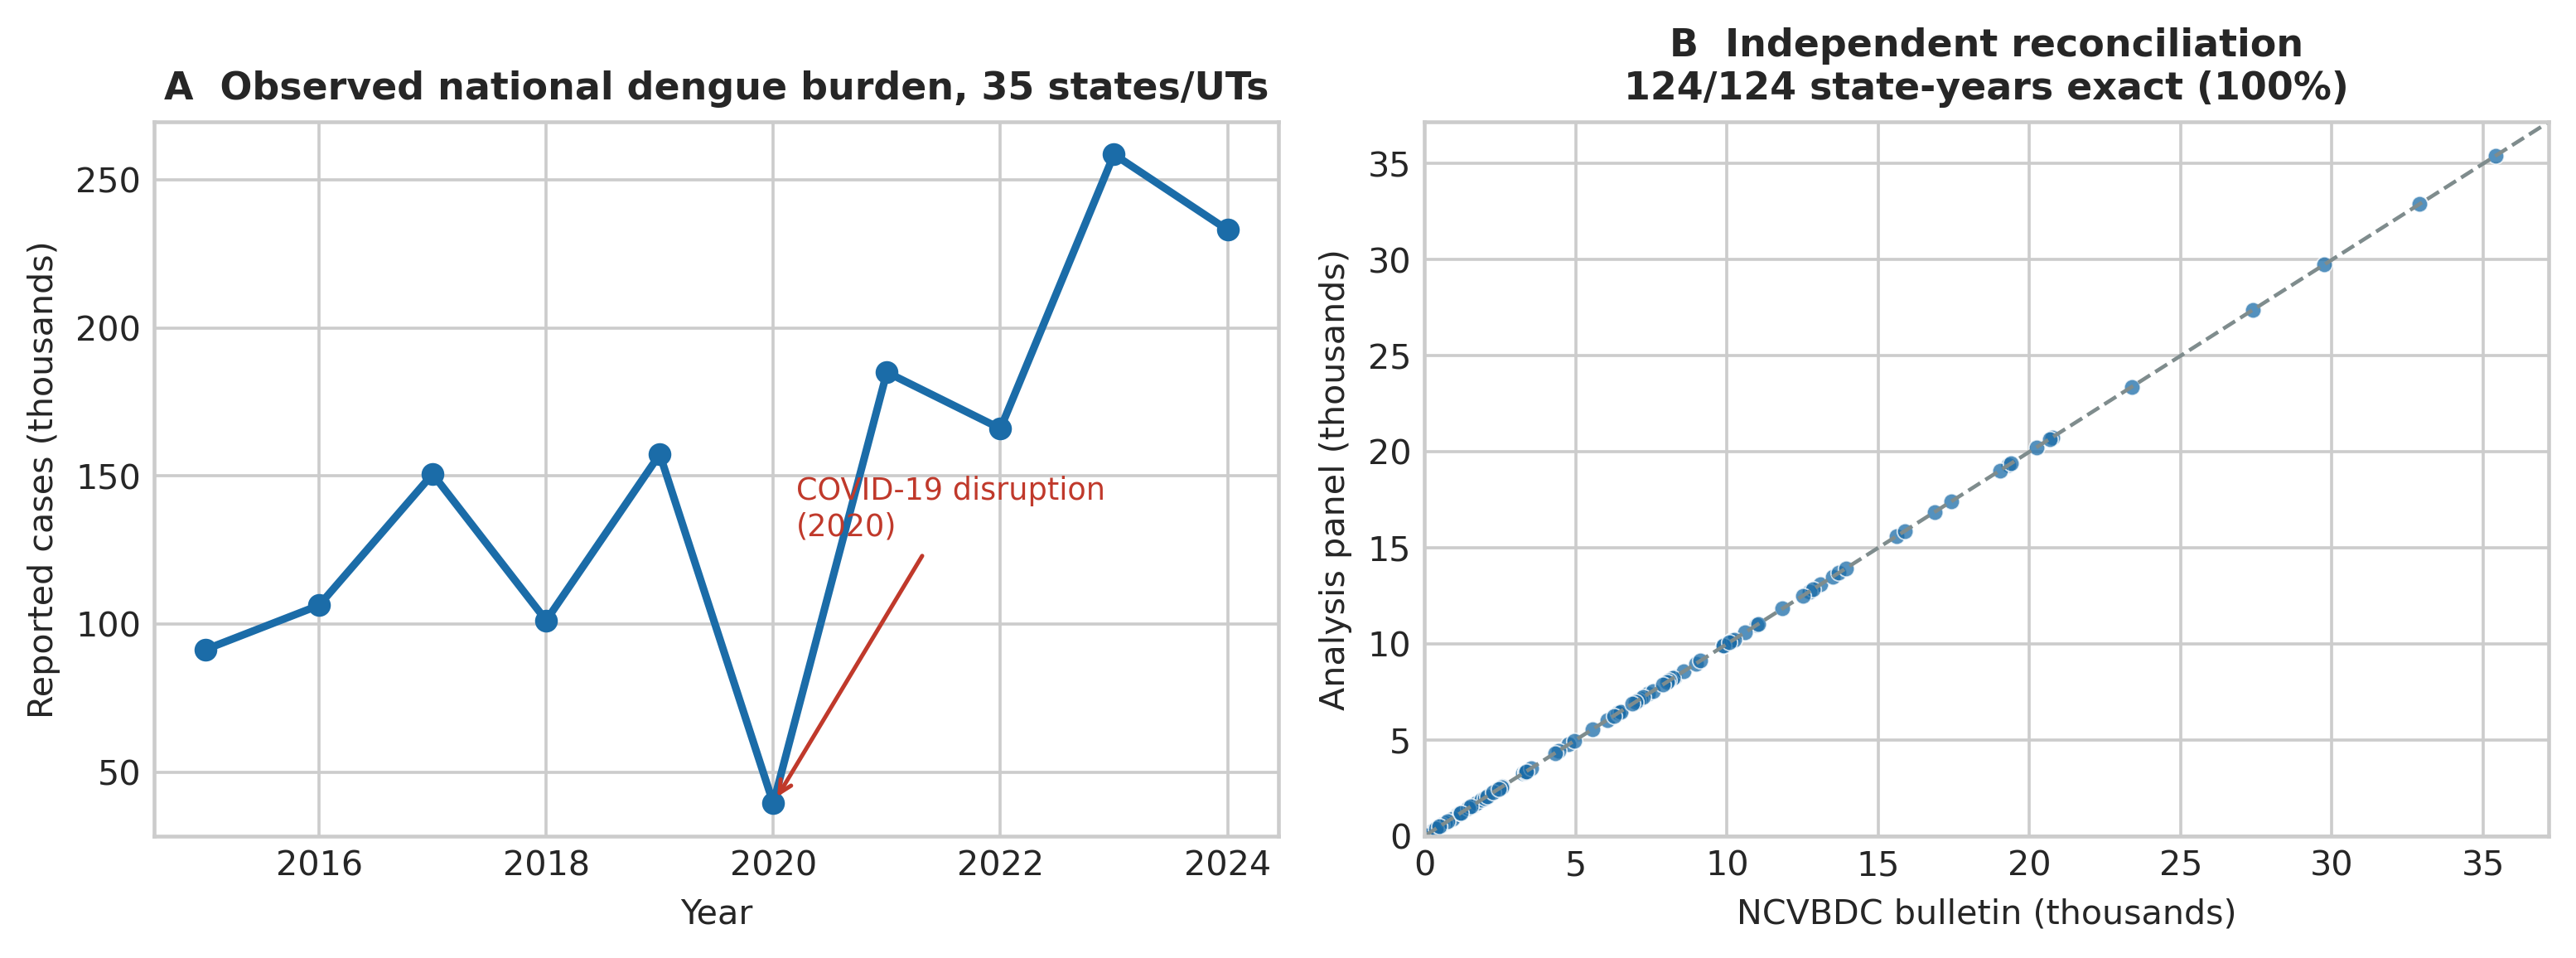
\includegraphics[keepaspectratio,alt={Figure 1. Panel provenance. (A) Observed annual reported dengue cases summed across the 35 states and union territories in the analysis panel, 2015--2024, showing the pronounced COVID-19 reporting disruption in 2020. (B) Independent reconciliation of the analysis panel against the NCVBDC state-wise annual bulletin for the 124 overlapping state-years; all values fall exactly on the identity line (100\% agreement).}]{figures/Figure1.png}}
\caption{Figure 1. Panel provenance. (A) Observed annual reported dengue
cases summed across the 35 states and union territories in the analysis
panel, 2015--2024, showing the pronounced COVID-19 reporting disruption
in 2020. (B) Independent reconciliation of the analysis panel against
the NCVBDC state-wise annual bulletin for the 124 overlapping
state-years; all values fall exactly on the identity line (100\%
agreement).}
\end{figure}

\begin{figure}
\centering
\pandocbounded{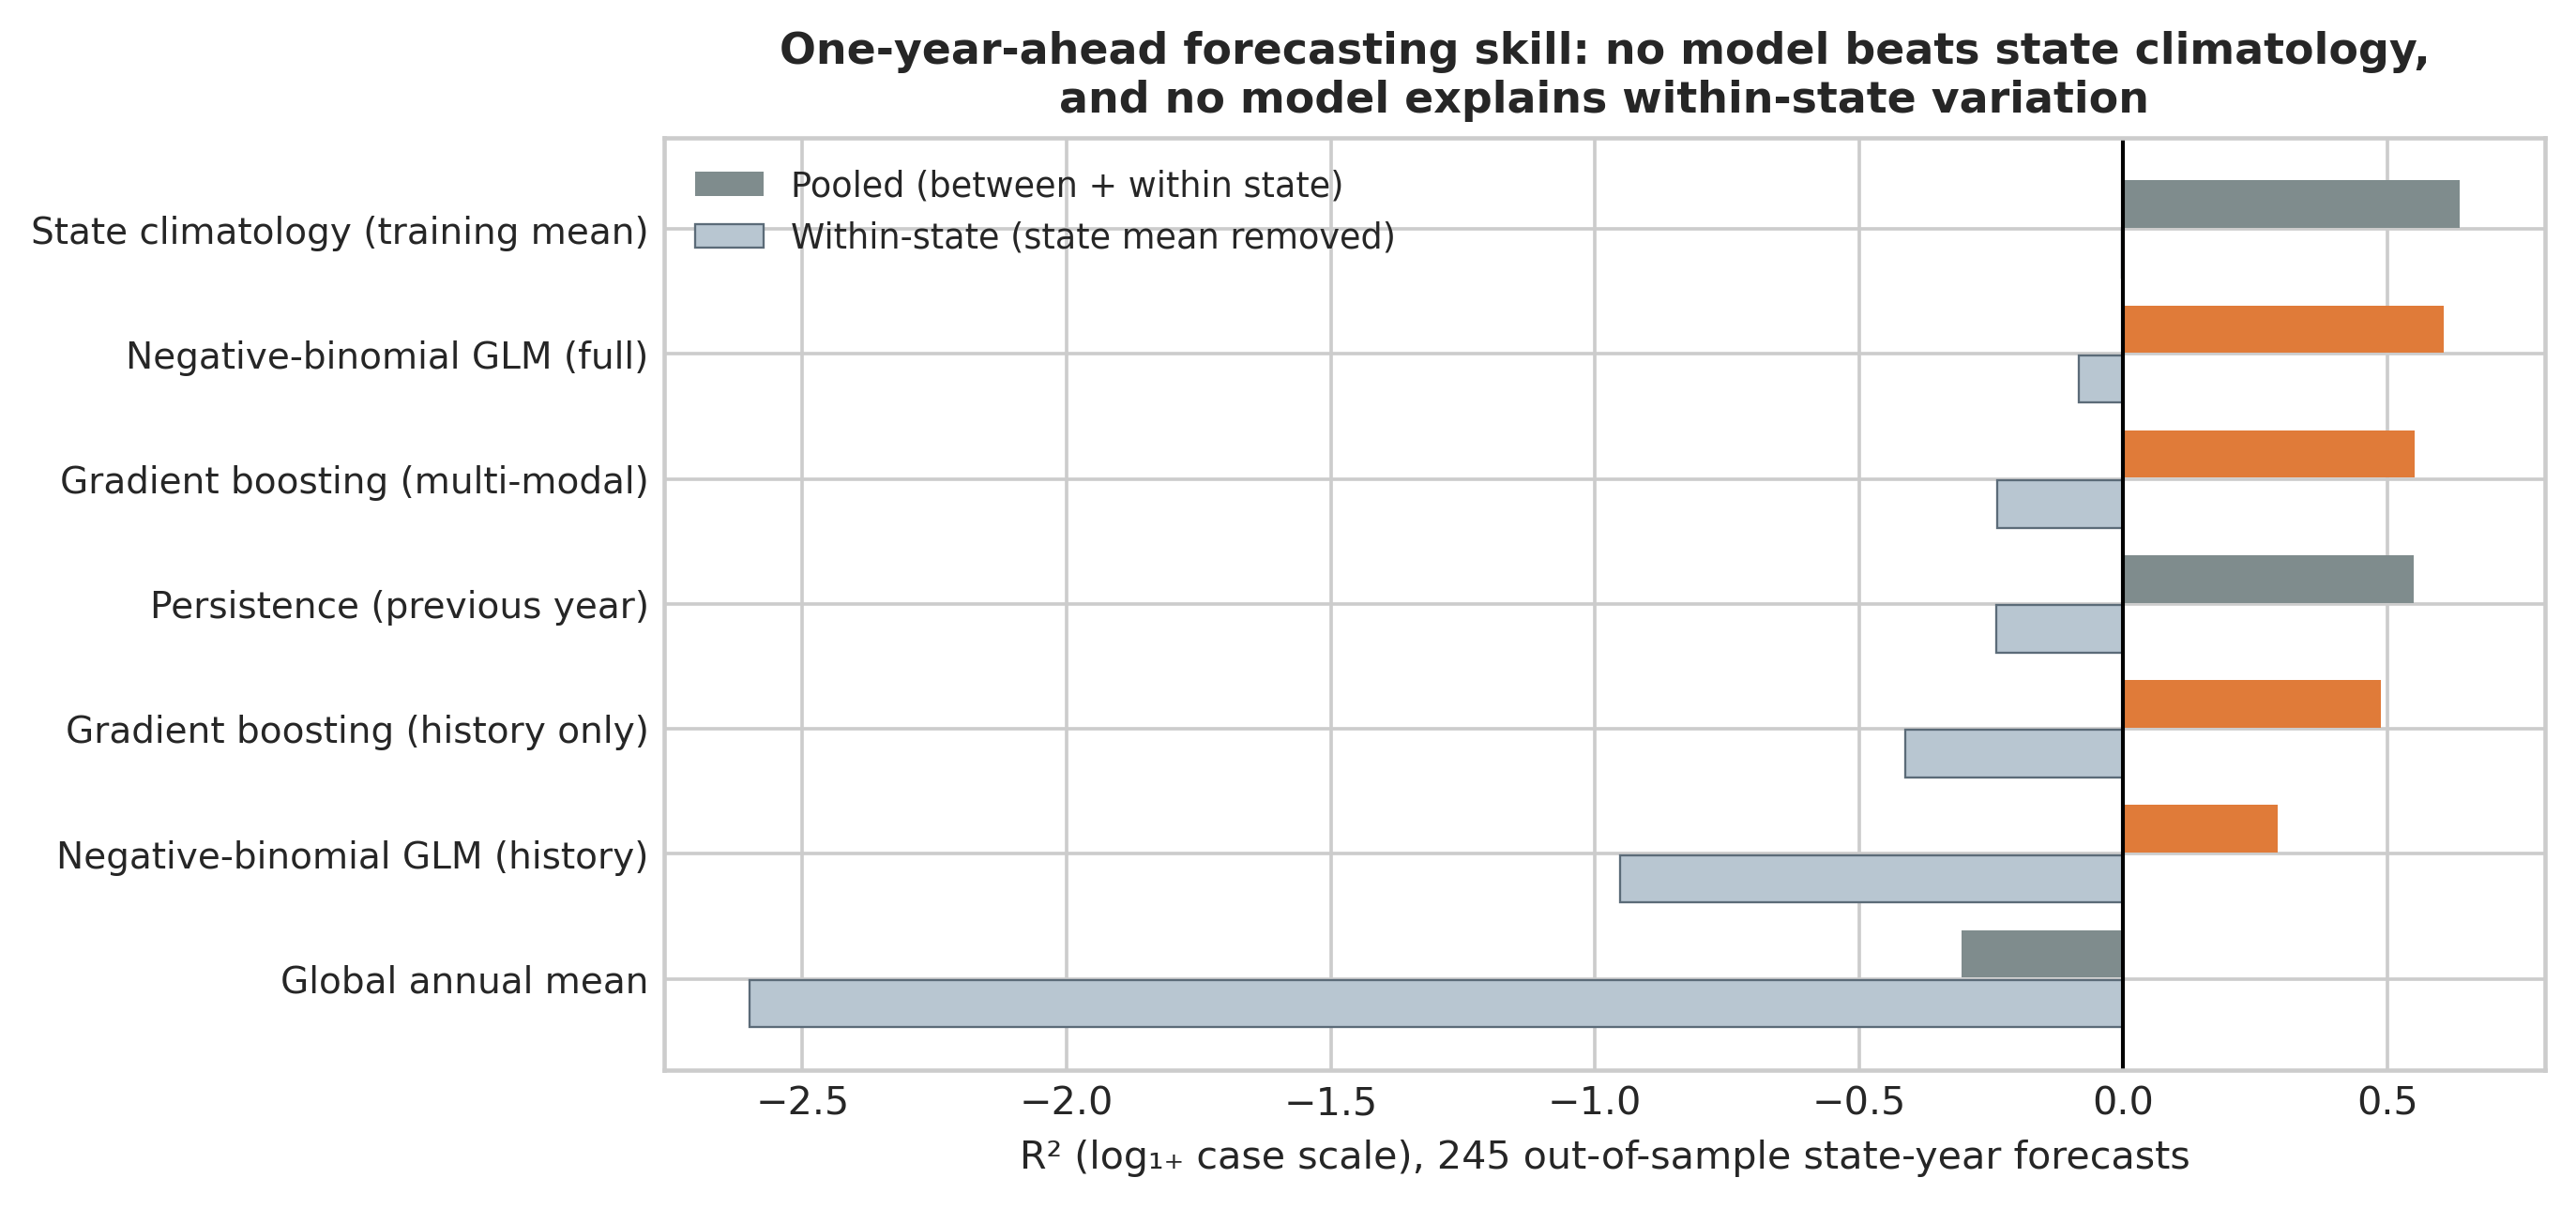
\includegraphics[keepaspectratio,alt={Figure 2. One-year-ahead forecasting skill across 245 out-of-sample state-year forecasts. Dark bars show pooled R²; light bars show within-state R² after removing each state's training-window mean. No model exceeds state climatology, and every within-state R² is at or below zero.}]{figures/Figure2.png}}
\caption{Figure 2. One-year-ahead forecasting skill across 245
out-of-sample state-year forecasts. Dark bars show pooled R²; light bars
show within-state R² after removing each state's training-window mean.
No model exceeds state climatology, and every within-state R² is at or
below zero.}
\end{figure}

\begin{figure}
\centering
\pandocbounded{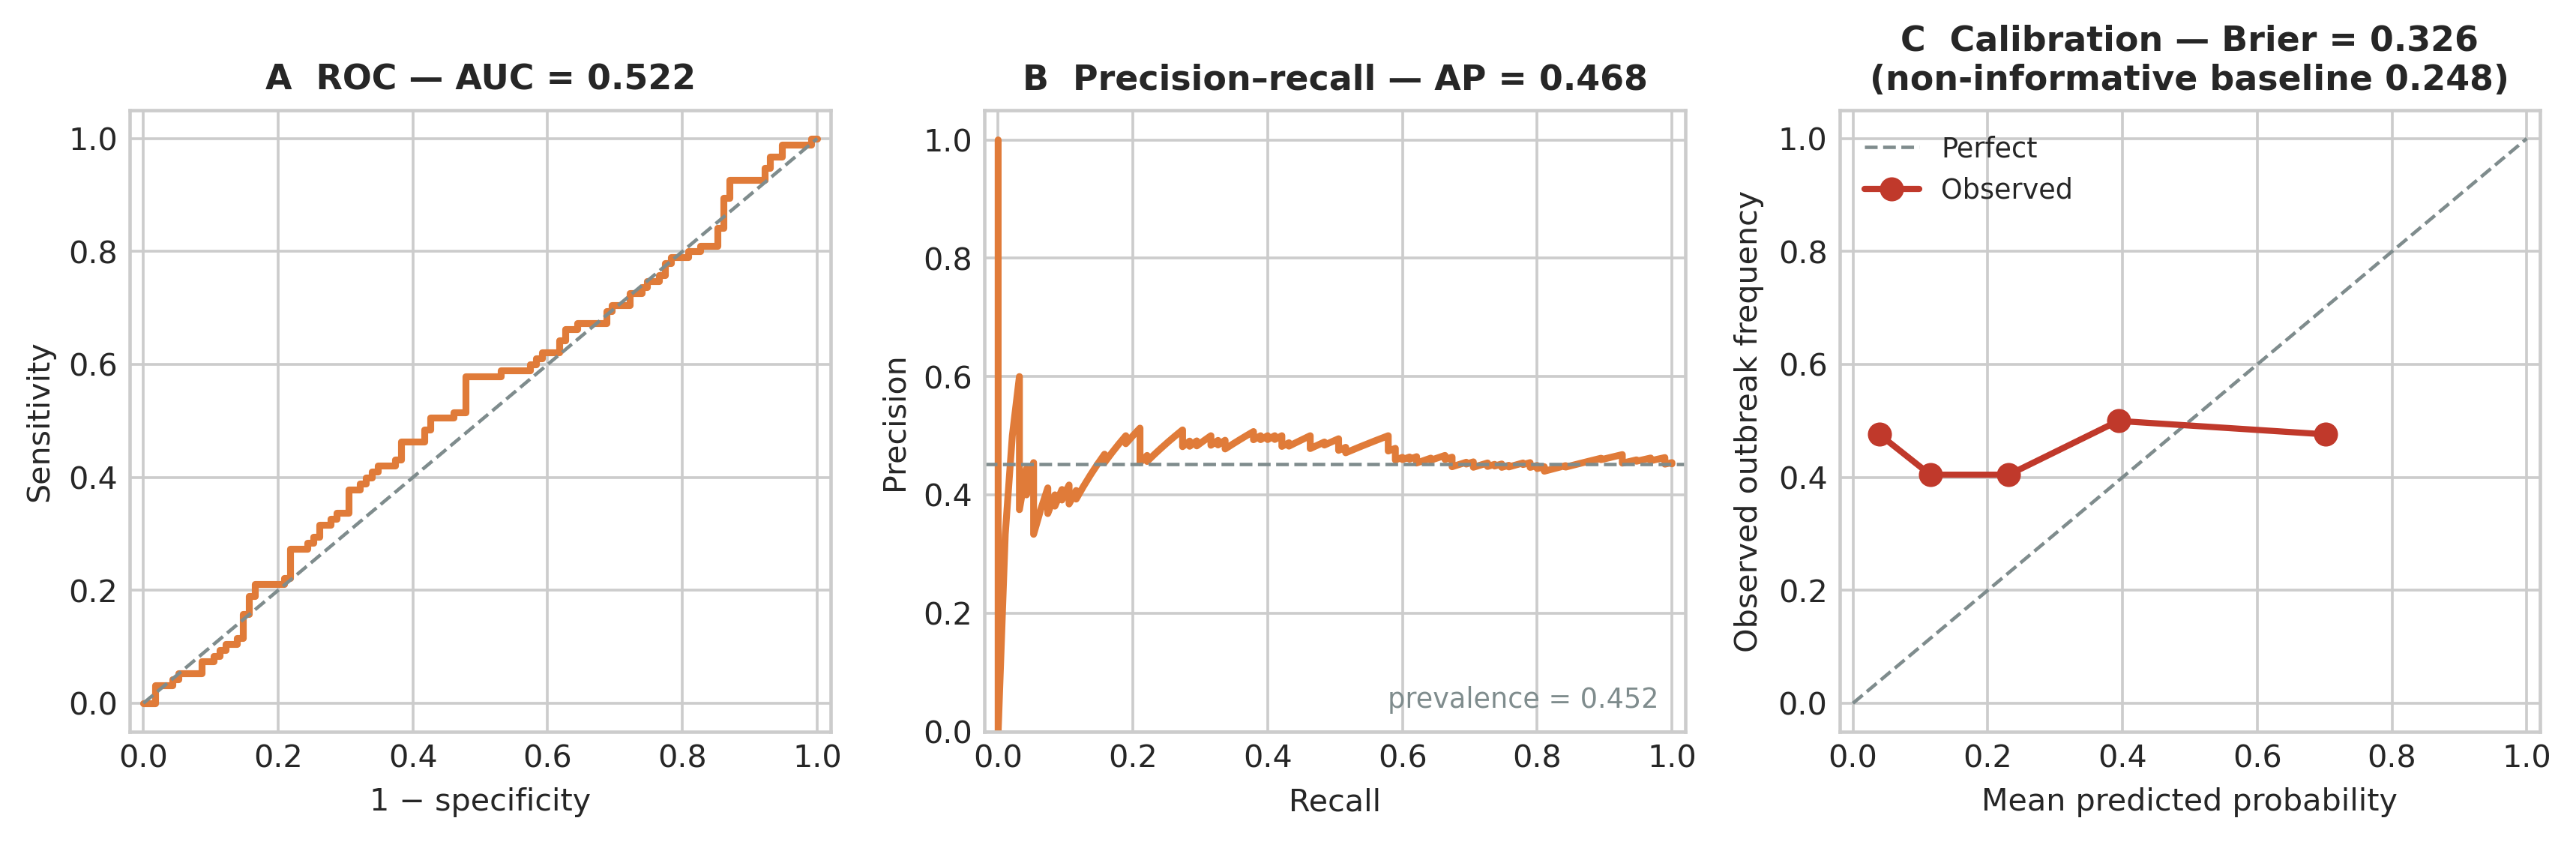
\includegraphics[keepaspectratio,alt={Figure 3. Outbreak-year classification. (A) ROC curve (AUC = 0.522). (B) Precision--recall curve against the observed prevalence of 0.452. (C) Quintile calibration curve; observed outbreak frequency is flat across predicted-probability quintiles and the Brier score (0.326) exceeds the non-informative baseline (0.248).}]{figures/Figure3.png}}
\caption{Figure 3. Outbreak-year classification. (A) ROC curve (AUC =
0.522). (B) Precision--recall curve against the observed prevalence of
0.452. (C) Quintile calibration curve; observed outbreak frequency is
flat across predicted-probability quintiles and the Brier score (0.326)
exceeds the non-informative baseline (0.248).}
\end{figure}

\begin{figure}
\centering
\pandocbounded{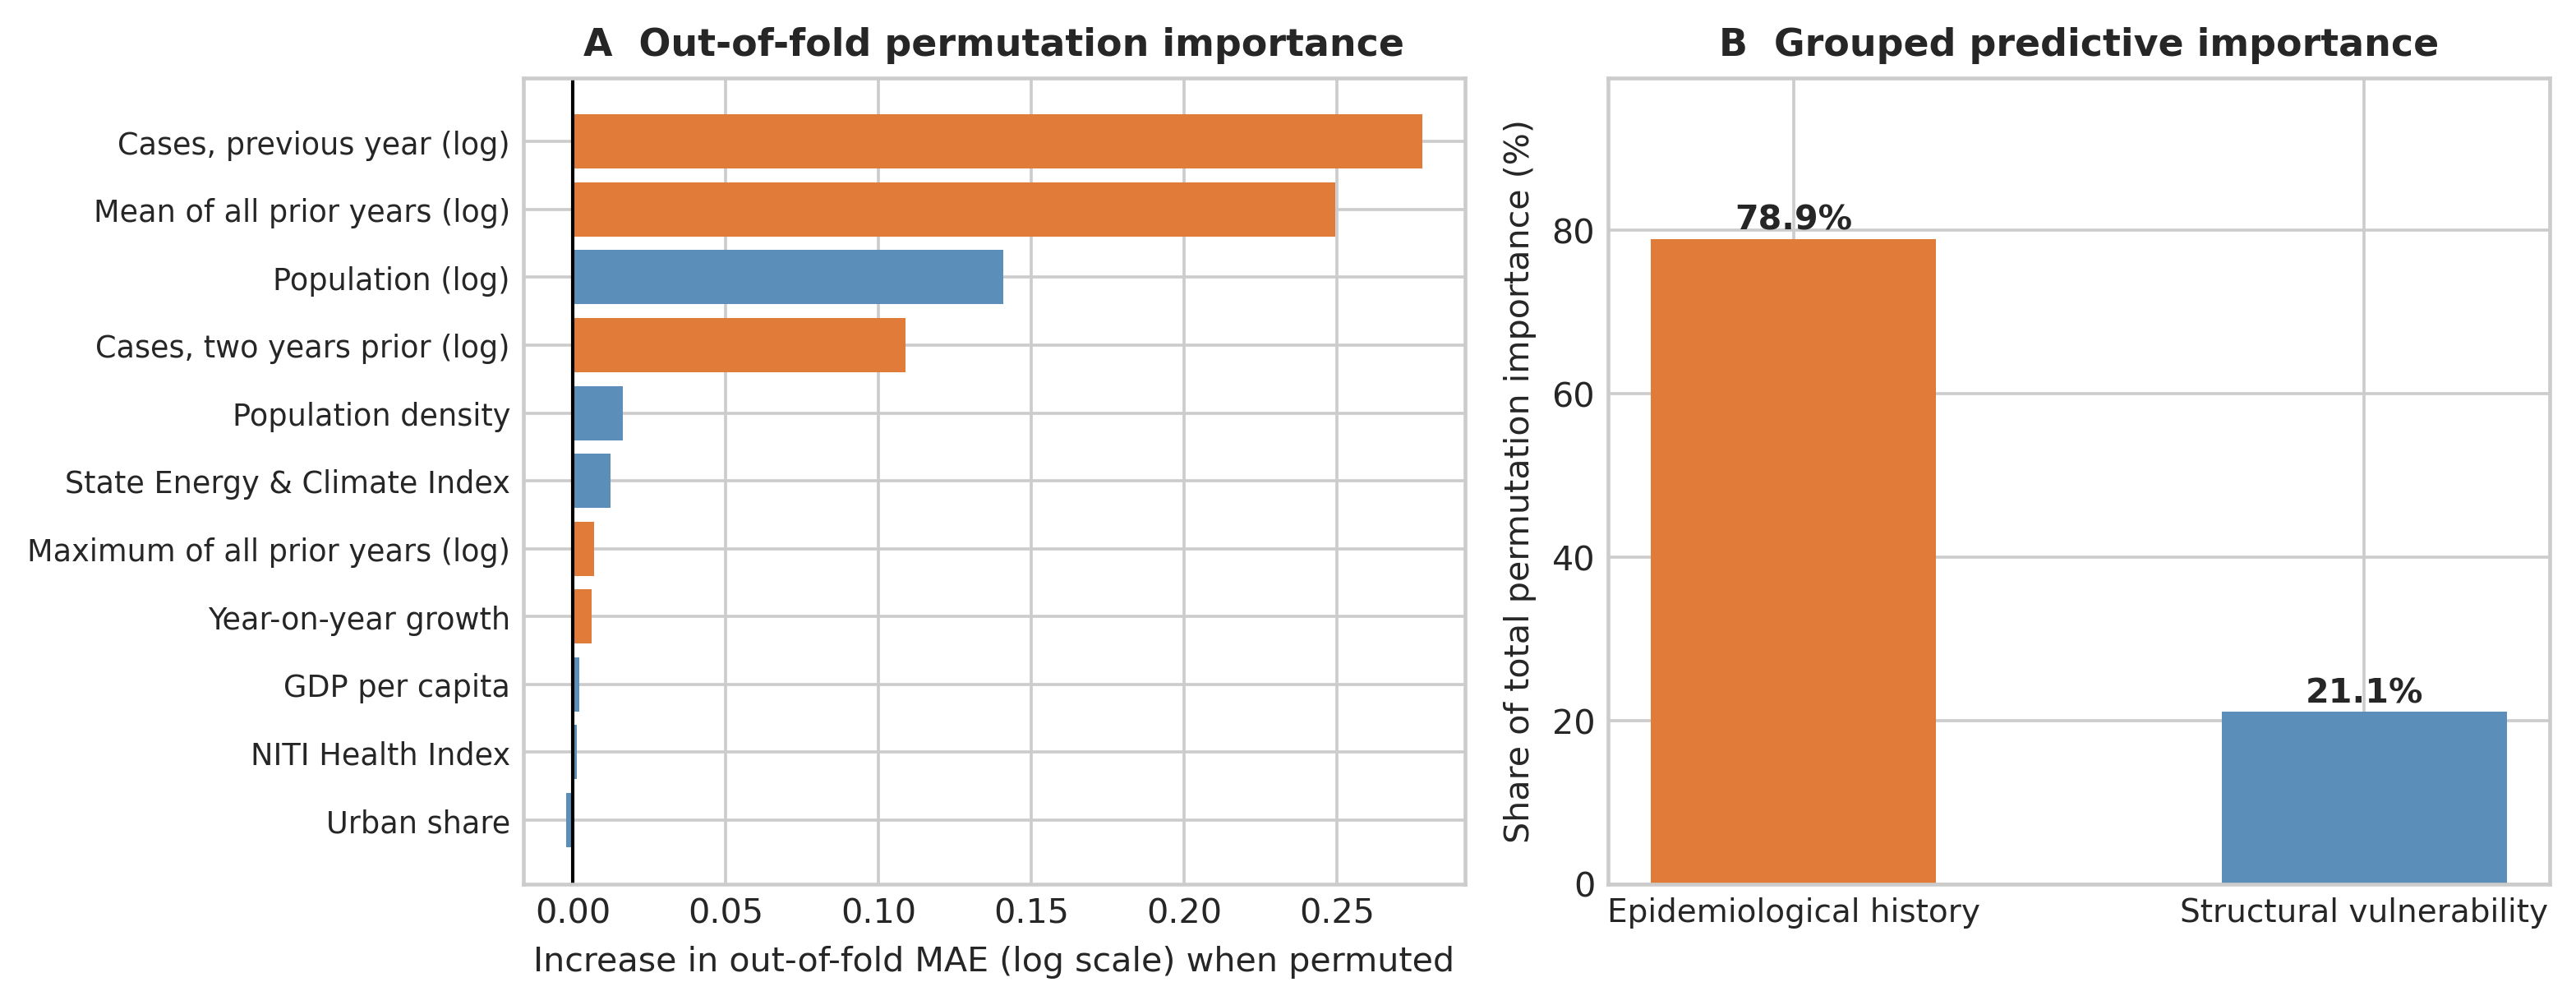
\includegraphics[keepaspectratio,alt={Figure 4. Out-of-fold permutation importance. (A) Increase in out-of-sample MAE when each predictor is permuted in the held-out year, averaged across forecast origins. (B) The same importances aggregated into epidemiological-history and structural-vulnerability blocks.}]{figures/Figure4.png}}
\caption{Figure 4. Out-of-fold permutation importance. (A) Increase in
out-of-sample MAE when each predictor is permuted in the held-out year,
averaged across forecast origins. (B) The same importances aggregated
into epidemiological-history and structural-vulnerability blocks.}
\end{figure}

\begin{figure}
\centering
\pandocbounded{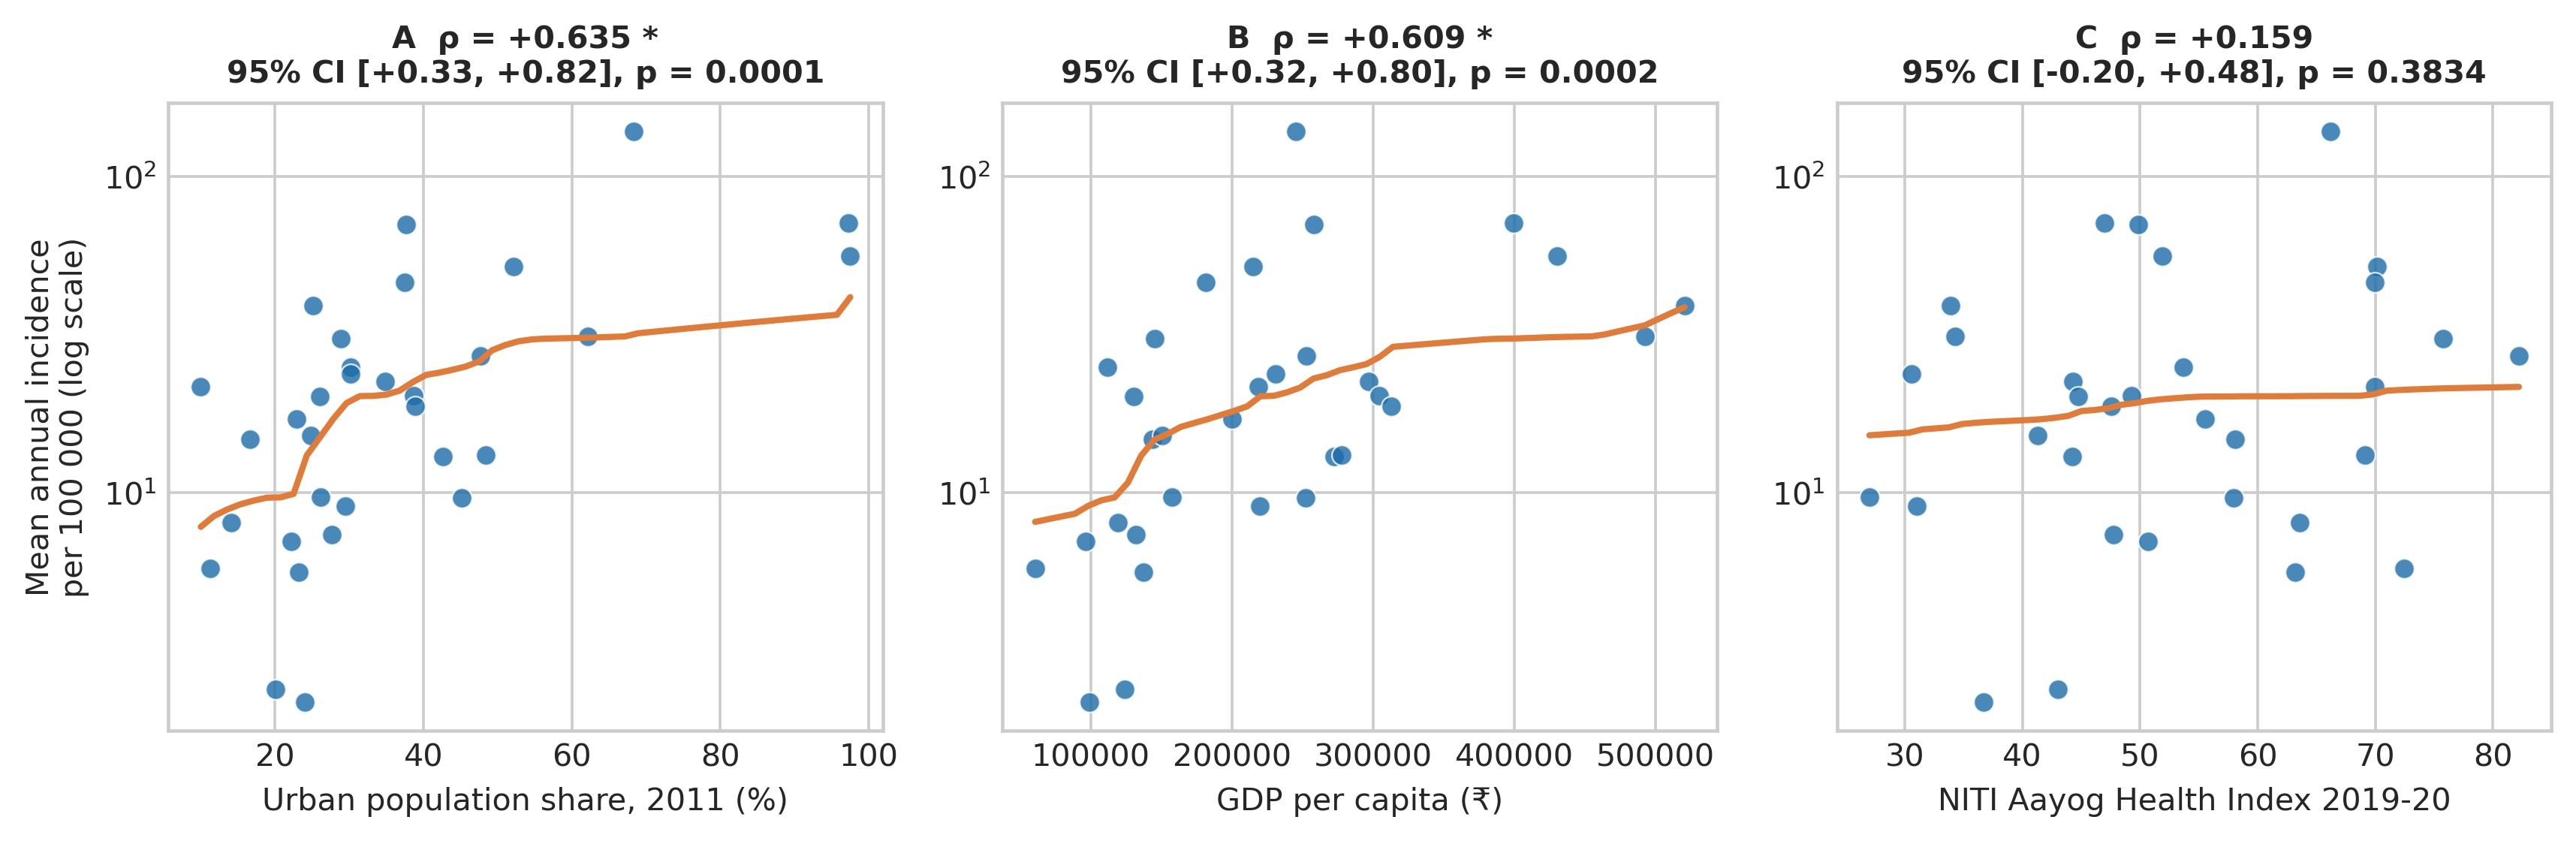
\includegraphics[keepaspectratio,alt={Figure 5. Between-state structural gradient in observed mean annual dengue incidence per 100 000 (log scale), 2015--2024, against (A) urban population share, (B) GDP per capita and (C) the NITI Aayog Health Index, with Spearman ρ, bootstrap 95\% CI and p-value.}]{figures/Figure5.png}}
\caption{Figure 5. Between-state structural gradient in observed mean
annual dengue incidence per 100 000 (log scale), 2015--2024, against (A)
urban population share, (B) GDP per capita and (C) the NITI Aayog Health
Index, with Spearman ρ, bootstrap 95\% CI and p-value.}
\end{figure}

\begin{figure}
\centering
\pandocbounded{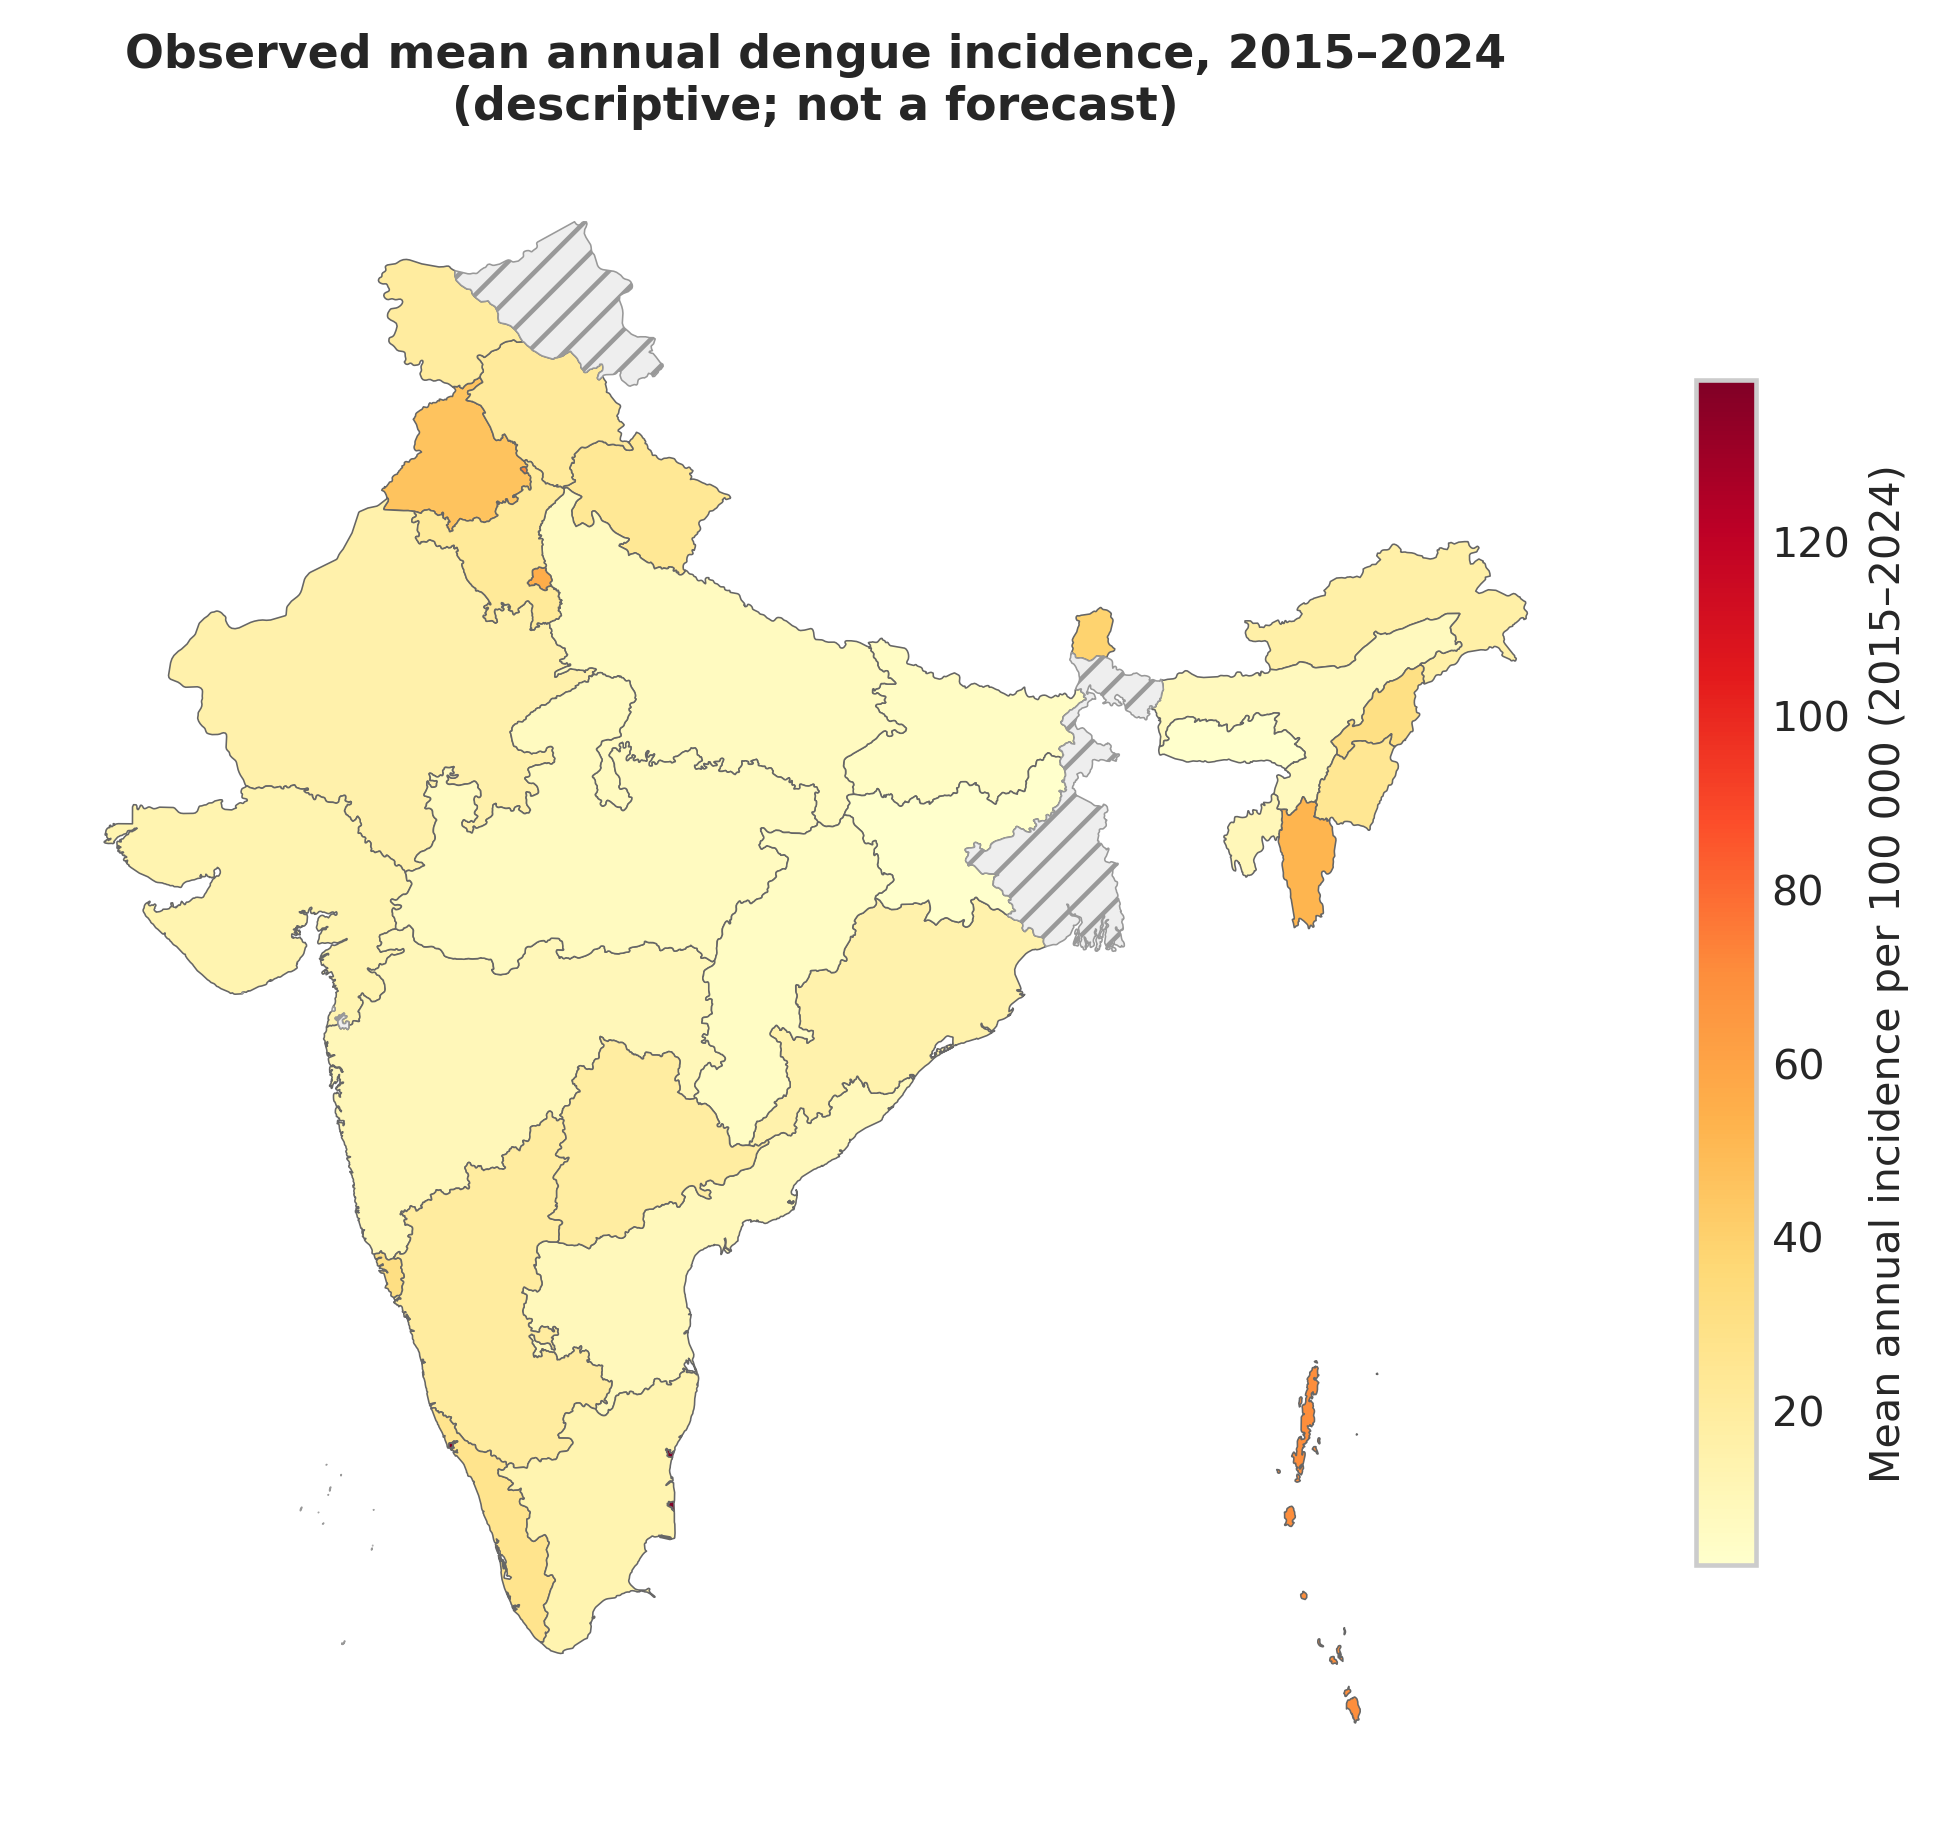
\includegraphics[keepaspectratio,alt={Figure 6. Descriptive choropleth of observed mean annual dengue incidence per 100 000 across the 35 panel states and union territories, 2015--2024. States not meeting the completeness criterion are hatched. This map is descriptive of observed burden and is not a forecast.}]{figures/Figure6.png}}
\caption{Figure 6. Descriptive choropleth of observed mean annual dengue
incidence per 100 000 across the 35 panel states and union territories,
2015--2024. States not meeting the completeness criterion are hatched.
This map is descriptive of observed burden and is not a forecast.}
\end{figure}

\begin{figure}
\centering
\pandocbounded{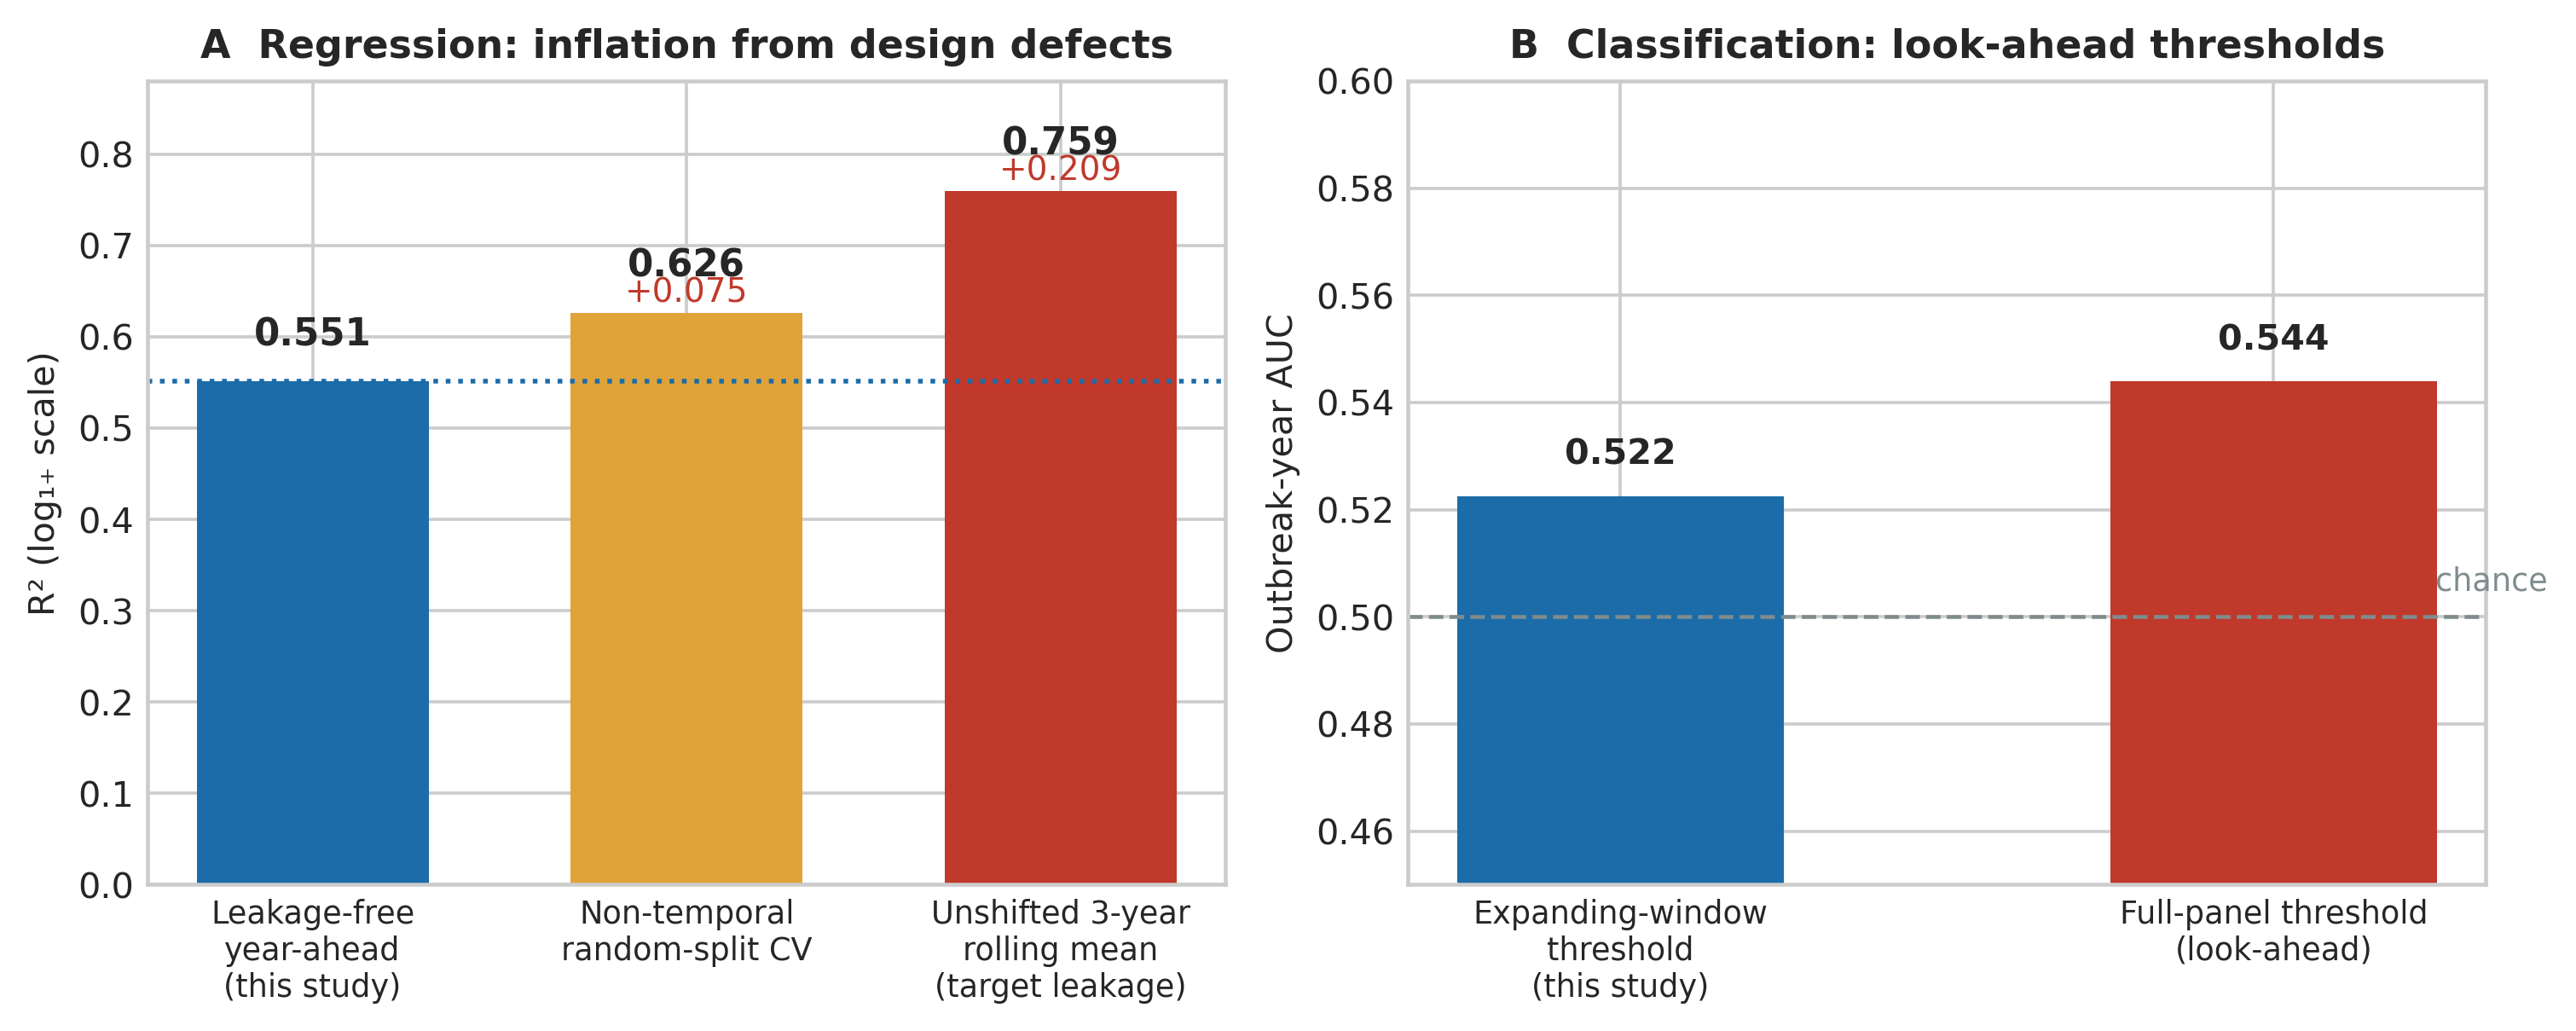
\includegraphics[keepaspectratio,alt={Figure 7. Leakage experiment on identical real data. (A) Apparent regression R² under the leakage-free design, under non-temporal random-split cross-validation, and after reintroducing an unshifted three-year rolling mean. (B) Outbreak-year AUC under expanding-window versus full-panel (look-ahead) outbreak thresholds.}]{figures/Figure7.png}}
\caption{Figure 7. Leakage experiment on identical real data. (A)
Apparent regression R² under the leakage-free design, under non-temporal
random-split cross-validation, and after reintroducing an unshifted
three-year rolling mean. (B) Outbreak-year AUC under expanding-window
versus full-panel (look-ahead) outbreak thresholds.}
\end{figure}

\subsection{8. References}\label{references}

\begin{enumerate}
\def\labelenumi{\arabic{enumi}.}
\item
  World Health Organization. \emph{Dengue} {[}Internet{]}. Geneva: World
  Health Organization; 2025 Aug 21 {[}cited 2026 Aug 20{]}. Available
  from:
  https://www.who.int/news-room/fact-sheets/detail/dengue-and-severe-dengue
\item
  Bhatt S, Gething PW, Brady OJ, Messina JP, Farlow AW, Moyes CL, et
  al.~The global distribution and burden of dengue. \emph{Nature}.
  2013;496(7446):504-507. doi:10.1038/nature12060.
\item
  Shepard DS, Halasa YA, Tyagi BK, et al.~Economic and disease burden of
  dengue illness in India. \emph{Am J Trop Med Hyg}.
  2014;91(6):1235-1242. doi:10.4269/ajtmh.14-0002.
\item
  National Centre for Vector Borne Diseases Control. \emph{Dengue
  Situation in India: Dengue Cases and Deaths in the Country}
  {[}Internet{]}. New Delhi: Directorate General of Health Services,
  Ministry of Health and Family Welfare, Government of India; {[}cited
  2026 Aug 20{]}. Available from:
  https://ncvbdc.mohfw.gov.in/index4.php?lang=1\&level=0\&lid=3715\&linkid=431
\item
  Lowe R, Stewart-Ibarra AM, Petrova D, García-Díez M, Borbor-Cordova
  MJ, Mejía R, et al.~Climate services for health: predicting the
  evolution of the 2016 dengue season in Machala, Ecuador. \emph{Lancet
  Planet Health}. 2017;1(4):e142-e151.
  doi:10.1016/S2542-5196(17)30064-5.
\item
  Salim NAM, Wah YB, Reeves C, Smith M, Yaacob WFW, Mudin RN, et
  al.~Prediction of dengue outbreak in Selangor Malaysia using machine
  learning techniques. \emph{Sci Rep}. 2021;11(1):939.
  doi:10.1038/s41598-020-79193-2.
\item
  Clarke J, Lim A, Gupte P, et al.~A global dataset of publicly
  available dengue case count data. \emph{Sci Data}. 2024;11:296.
  doi:10.1038/s41597-024-03120-7. Data extract used: OpenDengue Spatial
  extract V1.3 {[}dataset{]}. Available from: https://opendengue.org
  {[}cited 2026 Aug 20{]}.
\item
  Kapoor S, Narayanan A. Leakage and the reproducibility crisis in
  machine-learning-based science. \emph{Patterns}. 2023;4(9):100804.
  doi:10.1016/j.patter.2023.100804.
\item
  NITI Aayog. \emph{Healthy States, Progressive India: Report on the
  Ranks of States and Union Territories---Health Index Round IV
  2019--20}. New Delhi: NITI Aayog, Government of India; 2021.
\item
  Collins GS, Moons KGM, Dhiman P, Riley RD, Beam AL, Van Calster B, et
  al.~TRIPOD+AI statement: updated guidance for reporting clinical
  prediction models that use regression or machine learning methods.
  \emph{BMJ}. 2024;385:e078378. doi:10.1136/bmj-2023-078378. Erratum in:
  \emph{BMJ}. 2024;385:q902. doi:10.1136/bmj.q902.
\item
  Tjaden NB, Thomas SM, Fischer D, Beierkuhnlein C. Extrinsic incubation
  period of dengue: knowledge, backlog, and applications of temperature
  dependence. \emph{PLoS Negl Trop Dis}. 2013;7(6):e2207.
  doi:10.1371/journal.pntd.0002207.
\item
  Friedman JH. Greedy function approximation: a gradient boosting
  machine. \emph{Ann Stat}. 2001;29(5):1189-1232.
  doi:10.1214/aos/1013203451.
\item
  Hicks SA, Strümke I, Thambawita V, Hammou M, Riegler MA, Halvorsen P,
  et al.~On evaluation metrics for medical applications of artificial
  intelligence. \emph{Sci Rep}. 2022;12:5979.
  doi:10.1038/s41598-022-09954-8.
\item
  Downey LE, Gadsden T, Del Rio Vilas V, Peiris D, Jan S. The impact of
  COVID-19 on essential health service provision for endemic infectious
  diseases in the South-East Asia region: a systematic review.
  \emph{Lancet Reg Health Southeast Asia}. 2022;1:100011.
  doi:10.1016/j.lansea.2022.100011.
\item
  Mutheneni SR, Morse AP, Caminade C, Upadhyayula SM. Dengue burden in
  India: recent trends and importance of climatic parameters.
  \emph{Emerg Microbes Infect}. 2017;6(8):e70. doi:10.1038/emi.2017.57.
\item
  Messina JP, Brady OJ, Golding N, Kraemer MUG, Wint GRW, Ray SE, et
  al.~The current and future global distribution and population at risk
  of dengue. \emph{Nat Microbiol}. 2019;4(9):1508-1515.
  doi:10.1038/s41564-019-0476-8.
\end{enumerate}

\end{document}
